
\documentclass[10pt,a4paper]{article}

% Om het totaal aantal pagina's te tellen
\usepackage{lastpage}
\usepackage{graphicx}

% Om de marges aan te passen
\usepackage[left=2cm,right=2cm,top=2cm,bottom=2cm]{geometry}

% Voor headers en footers
\usepackage{fancyhdr}
\pagestyle{fancy}

\lhead{Giuseppe Callari and Xavier Go\'as Aguililla}
\rhead{\thepage /\pageref{LastPage}}

\lfoot{Assignment}
\cfoot{Computer Networks}
\rfoot{Network Simulation}

\renewcommand{\headrulewidth}{0.4pt}
\renewcommand{\footrulewidth}{0.4pt}

\begin{document}
\begin{titlepage}
\thispagestyle{empty}
\newcommand{\HRule}{\rule{\linewidth}{0.5mm}}
\center
\textsc{\LARGE KU Leuven}\\[1.5cm]
\textsc{\Large Assignment:}\\[0.5cm]
\textsc{\large Network Simulation}\\[0.5cm]

\HRule \\[0.4cm]
{ \Huge \bfseries Report}\\[0.4cm]
\HRule \\[1.5cm]

\begin{minipage}{0.4\textwidth}
\begin{flushleft} \large
\emph{Authors:}\\
Giuseppe \textsc{Callari}\\
Xavier \textsc{Go\'as Aguililla}
\end{flushleft}
\end{minipage}
~
\begin{minipage}{0.4\textwidth}
\begin{flushright} \large
\emph{Professor:} \\
prof. dr. D. \textsc{Hughes}
\end{flushright}
\end{minipage}\\[4cm]

{\large May 2nd, 2014}\\[3cm]
\vfill

\end{titlepage}


\section{Exercise 1}
\subsection{Question 1}
In figure \ref{fig:lala} we can clearly see the difference between the
scenario with both an uploader and a downloader and that without an
uploader. In the scenario with an uploader, around the time the upload
starts (3.0s), the throughput for the downloader drops drastically. In
the scenario without an uploader, indicated in green, the throughput
of the connection remains roughly constant.

\begin{figure}[p]
    \centering
    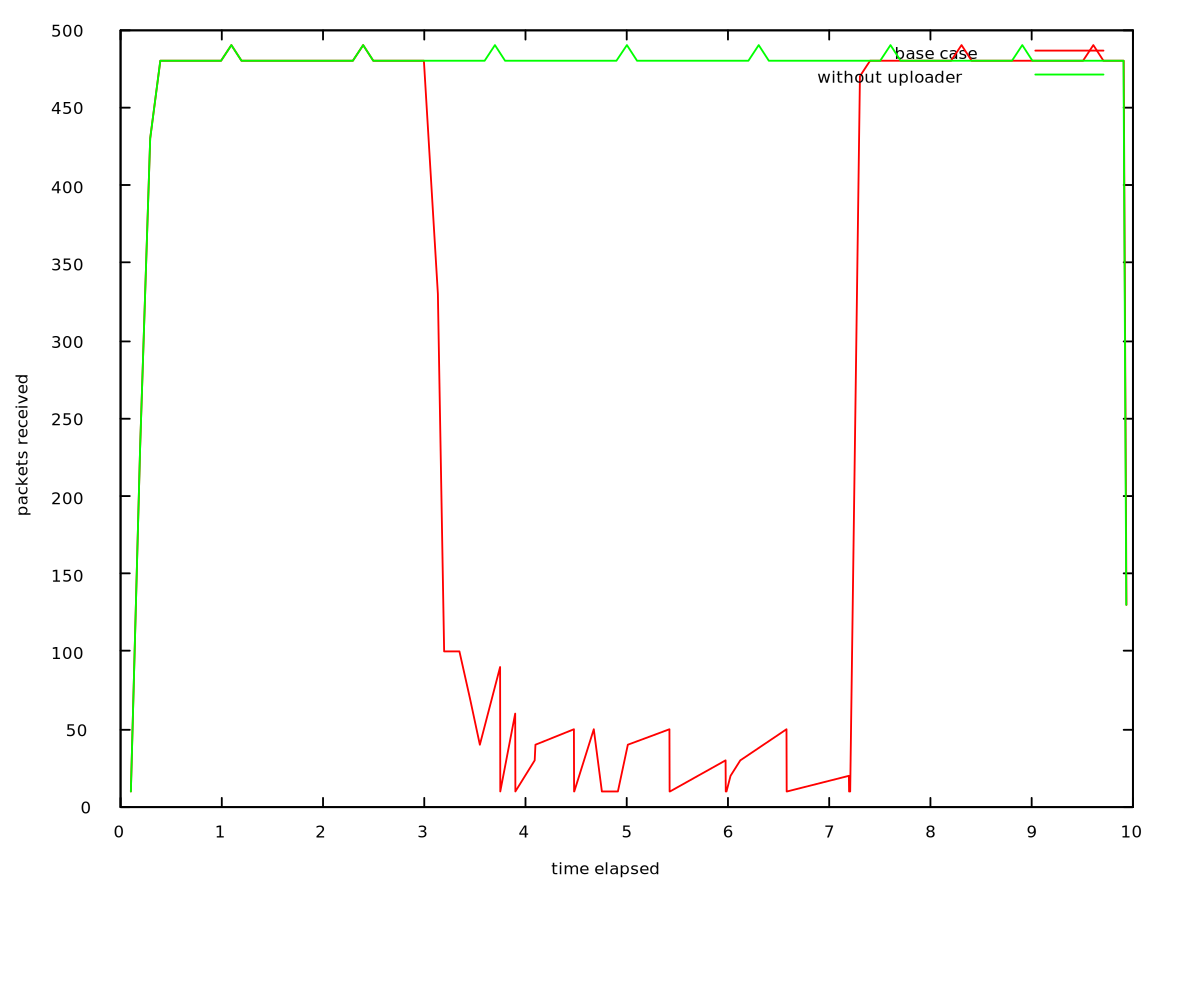
\includegraphics[width=\textwidth]{../part1/q1/plots/1.pdf}
    \caption{Download throughput compared}
    \label{fig:lala}
\end{figure}

\subsection{Question 2}
In figure \ref{fig:combined1} we see both the upload and download
throughput on the same graph; we can clearly see the aforementioned
drop in download speed at the moment the upload over CBR starts.

\begin{figure}[p]
    \centering
    \includegraphics[width=\textwidth]{../part1/q2/plots/2.pdf}
    \caption{Upload and download throughput}
    \label{fig:combined1}
\end{figure}
\subsection{Question 3}

We expect performance for CBR to be excellent, since a certain amount
of bandwidth is always guaranteed for the upload connection. This does
imply that the upload connection has a certain privilege over the
download connection; to ensure this, we could tell the router to drop
downstream packets rather than upstream packets. This would result in
increased packet loss for the download connection, especially if we
would run multiple upload connections at the same time.

\subsection{Question 4}

We can see in \ref{down_limited}

We can see in \ref{up_limited}

\begin{figure}[p]
    \centering
    \includegraphics[width=\textwidth]{../part1/q4/plots/4-down.pdf}
    \caption{Download throughput}
    \label{fig:down_limited}
\end{figure}

\begin{figure}[p]
    \centering
    \includegraphics[width=\textwidth]{../part1/q4/plots/4-up.pdf}
    \caption{Upload throughput}
    \label{fig:up_limited}
\end{figure}

\subsection{Question 5}
\subsection{Question 6}

\section{Exercise 2}
\subsection{Question 1}
\subsection{Question 2}
\subsection{Question 3}
\subsection{Question 4}

\end{document}